
%DIF LATEXDIFF DIFFERENCE FILE
%DIF DEL .\Math-7081.tex             Wed May 24 22:42:16 2023
%DIF ADD .\Math-7081-corrected.tex   Thu May 25 22:47:46 2023
\documentclass{aims}
\usepackage{txfonts, verbatim}
\usepackage{amsmath}	
\usepackage{flexisym, breqn}	
\usepackage{amssymb, graphics, setspace}	
\usepackage{tikz, tikz-cd}	
\usepackage{flowchart}	
\usepackage{float, booktabs}	
\usepackage{algorithmicx, algorithm,algpseudocode}	
\usepackage{blindtext}	
\usepackage{url}	
\usepackage[pagewise]{lineno}
\usepackage[comma, square, sort, numbers]{natbib}

\usetikzlibrary{positioning, cd, arrows, celtic}	%% for comutative diagram & flowchart drawing

\renewcommand{\bibnumfmt}[1]{#1.}

\def\typeofarticle{Research article}
\def\currentvolume{8}
\def\currentissue{8}
\def\currentyear{2023}
\def\currentmonth{}
\def\ppages{xxxx--xxxx.}
\def\DOI{ 10.3934/math.2023xxx}
\def\Received{08 January 2023}
\def\Revised{29 April 2023}
\def\Accepted{19 May 2023}
\def\Published{x May 2023}
\setcounter{page}{1}
\hyphenpenalty=10000
%\usepackage{cite}
\captionsetup[figure]{font=normalsize,labelfont=bf,singlelinecheck=true}
\captionsetup[table]{font=normalsize,labelfont=bf,singlelinecheck=true}



\numberwithin{equation}{section}
\DeclareMathOperator*{\essinf}{ess\,inf}
\makeatletter
\renewcommand{\@biblabel}[1]{#1\hfill \hspace{-0.2cm}}
\makeatother

\newcommand{\ep}{\varepsilon}
\newcommand{\eps}[1]{{#1}_{\varepsilon}}

\newtheorem{theorem}{Theorem}	%% definition for theorem env
\newtheorem{axiom}{Axiom}	%% definition for axiom env
\newtheorem{definition}{Definition}	%% definition for definition env

\numberwithin{theorem}{section}	%% count theorems
\numberwithin{axiom}{section}	%% count axioms
\numberwithin{definition}{section}	%% count definitions
%DIF PREAMBLE EXTENSION ADDED BY LATEXDIFF
%DIF UNDERLINE PREAMBLE %DIF PREAMBLE
\RequirePackage[normalem]{ulem} %DIF PREAMBLE
\RequirePackage{color}\definecolor{RED}{rgb}{1,0,0}\definecolor{BLUE}{rgb}{0,0,1} %DIF PREAMBLE
\providecommand{\DIFadd}[1]{{\protect\color{blue}\uwave{#1}}} %DIF PREAMBLE
\providecommand{\DIFdel}[1]{{\protect\color{red}\sout{#1}}}                      %DIF PREAMBLE
%DIF SAFE PREAMBLE %DIF PREAMBLE
\providecommand{\DIFaddbegin}{} %DIF PREAMBLE
\providecommand{\DIFaddend}{} %DIF PREAMBLE
\providecommand{\DIFdelbegin}{} %DIF PREAMBLE
\providecommand{\DIFdelend}{} %DIF PREAMBLE
\providecommand{\DIFmodbegin}{} %DIF PREAMBLE
\providecommand{\DIFmodend}{} %DIF PREAMBLE
%DIF FLOATSAFE PREAMBLE %DIF PREAMBLE
\providecommand{\DIFaddFL}[1]{\DIFadd{#1}} %DIF PREAMBLE
\providecommand{\DIFdelFL}[1]{\DIFdel{#1}} %DIF PREAMBLE
\providecommand{\DIFaddbeginFL}{} %DIF PREAMBLE
\providecommand{\DIFaddendFL}{} %DIF PREAMBLE
\providecommand{\DIFdelbeginFL}{} %DIF PREAMBLE
\providecommand{\DIFdelendFL}{} %DIF PREAMBLE
%DIF COLORLISTINGS PREAMBLE %DIF PREAMBLE
\RequirePackage{listings} %DIF PREAMBLE
\RequirePackage{color} %DIF PREAMBLE
\lstdefinelanguage{DIFcode}{ %DIF PREAMBLE
%DIF DIFCODE_UNDERLINE %DIF PREAMBLE
  moredelim=[il][\color{red}\sout]{\%DIF\ <\ }, %DIF PREAMBLE
  moredelim=[il][\color{blue}\uwave]{\%DIF\ >\ } %DIF PREAMBLE
} %DIF PREAMBLE
\lstdefinestyle{DIFverbatimstyle}{ %DIF PREAMBLE
	language=DIFcode, %DIF PREAMBLE
	basicstyle=\ttfamily, %DIF PREAMBLE
	columns=fullflexible, %DIF PREAMBLE
	keepspaces=true %DIF PREAMBLE
} %DIF PREAMBLE
\lstnewenvironment{DIFverbatim}{\lstset{style=DIFverbatimstyle}}{} %DIF PREAMBLE
\lstnewenvironment{DIFverbatim*}{\lstset{style=DIFverbatimstyle,showspaces=true}}{} %DIF PREAMBLE
%DIF END PREAMBLE EXTENSION ADDED BY LATEXDIFF

\begin{document}
	\title{A new type of generic, self-evolving and efficient automated deduction algorithm based on category theory}
	\author{%
		Zijian Wang\affil{1}
		and Xinhui Shao\affil{2,*}
	}
	\shortauthors{the Authors}
	\DIFdelbegin %DIFDELCMD < \address{%
%DIFDELCMD < 		\addr{\affilnum{1}}{Northeast Yucai School, Zhenxing St. 9-5, Heping District, Shenyang, Liaoning, China.}
%DIFDELCMD < 		\addr{\affilnum{2}}{Department of Mathematics, College of Sciences, Northerneastern University, Shenyang, Liaoning, China. }
%DIFDELCMD < 		\corraddr{Email: shaoxinhui@mail.neu.edu.cn.}
%DIFDELCMD < 	}
%DIFDELCMD < %%%
\DIFdelend \DIFaddbegin \address{%
		\addr{\affilnum{1}}{Northeast Yucai School, Zhenxing St. 9-5, Heping District, Shenyang, Liaoning, China.}
		\addr{\affilnum{2}}{Department of Mathematics, College of Sciences, Northeastern University, Shenyang, Liaoning, China. }
		\corraddr{Email: shaoxinhui@mail.neu.edu.cn.}
	}
\DIFaddend 

	\begin{abstract}
	In this article\DIFaddbegin \DIFadd{, }\DIFaddend a new type of generalized, self-evolving and efficient automated statement proof algorithm based on new data structures, i.e., brackets and map graphs\DIFaddbegin \DIFadd{,
	}\DIFaddend and new algorithms is presented. The brackets structure provides an elegant low-knowledge representation of mathematical concepts. The map graphs offer an efficient machine-learning method which let the computer learn knowledge while proving. Additionally, the new finding is  \DIFdelbegin \DIFdel{totally built on the }\DIFdelend \DIFaddbegin \DIFadd{built completely on }\DIFaddend category theory. Furthermore, a prototype of the program is \DIFdelbegin \DIFdel{given }\DIFdelend \DIFaddbegin \DIFadd{presented }\DIFaddend and examined for performance.
	\end{abstract}

	\keywords{
		{automatic prover; theorem prover; algorithm; category theory; automatic deduction; automatic reasoning}
		\newline
		\textbf{Mathematics Subject Classification:} 03B35, 68V15, 18-00, 18-04, 68W99
	}

	\maketitle

	\section{Introduction}
	During the long period of development \DIFdelbegin \DIFdel{of the }\DIFdelend \DIFaddbegin \DIFadd{and }\DIFaddend research on automated theorem provers, there have already existed a great number of research and implementation on proofs focusing on a specific mathematical subject, such as \DIFdelbegin \DIFdel{algebra }\DIFdelend \DIFaddbegin \DIFadd{algebraic }\DIFaddend equations (for example, Wolfram Mathematica{'}s Find Equation Proof function \cite{Wolfram2019}) or geometrical theorems (for example, the Geometry Expert or GEX \cite{Gao1998} of Key Laboratory of Mathematics Mechanization, Chinese Academy of Sciences). Some relatively new works in this aspect \DIFdelbegin \DIFdel{includes }\DIFdelend \DIFaddbegin \DIFadd{included }\DIFaddend Microsoft{'}s Lean prover \cite{Moura2021} and \DIFaddbegin \DIFadd{the }\DIFaddend Z3 \cite{Moura2008} algorithm.

	However, if we investigate deeper into these algorithms, we will find the fact that all of these provers stand on the basis of logic theories. Both completely automated theorem provers and semi-automated computer auxiliary statement provers like Coq and Isabelle \DIFdelbegin \DIFdel{, }\DIFdelend are designed to follow certain logic rules and generate results as logic formulas. Nevertheless, although we have to admit that \DIFdelbegin \DIFdel{such do }\DIFdelend \DIFaddbegin \DIFadd{it }\DIFaddend is an effective method, this method also sets an insurmountable limit on the \DIFdelbegin \DIFdel{execution that the program could }\DIFdelend \DIFaddbegin \DIFadd{program that it can }\DIFaddend not think comprehensively such as \DIFaddbegin \DIFadd{when }\DIFaddend solving an algebra problem in a geometrical way.

	When we humans think of mathematical problems and perform proofs, we do not follow purely logical \DIFdelbegin \DIFdel{ways like complex stuff like }\DIFdelend \DIFaddbegin \DIFadd{methods, for example, by executing the }\DIFaddend Cooper{'}s algorithm. Instead, we \DIFdelbegin \DIFdel{just perform tries }\DIFdelend \DIFaddbegin \DIFadd{attempt }\DIFaddend to seek breakthrough points using \DIFdelbegin \DIFdel{his knowledge in a diversified }\DIFdelend \DIFaddbegin \DIFadd{our knowledge and diverse }\DIFaddend thought. Why \DIFdelbegin \DIFdel{cannot programs }\DIFdelend \DIFaddbegin \DIFadd{can programs not }\DIFaddend do things like that? Why can not they perform some sort of knowledge \DIFdelbegin \DIFdel{transferring? Carry this question and in experimental and curious attitude}\DIFdelend \DIFaddbegin \DIFadd{transfer? Interested in these questions}\DIFaddend , we conducted \DIFdelbegin \DIFdel{the }\DIFdelend research on this topic and have found a utility to \DIFdelbegin \DIFdel{do }\DIFdelend \DIFaddbegin \DIFadd{perform }\DIFaddend the task: \DIFdelbegin \DIFdel{The category }\DIFdelend \DIFaddbegin \DIFadd{Category }\DIFaddend theory.

	Mainly developed in the twentieth century by \DIFdelbegin \DIFdel{the contribution of MacLane }\DIFdelend \DIFaddbegin \DIFadd{Mac Lane }\DIFaddend and Eilenberg with the purpose \DIFdelbegin \DIFdel{to investigate algebra topology, the category theory is }\DIFdelend \DIFaddbegin \DIFadd{of investigating algebraic topology, category theory has become }\DIFaddend a fast-evolving aspect of modern mathematics. In just a few decades, \DIFdelbegin \DIFdel{the }\DIFdelend category theory has become the standard and formal language of homology algebra and algebraic geometry\DIFdelbegin \DIFdel{and has gained a lot of }\DIFdelend \DIFaddbegin \DIFadd{, and has contributed to many }\DIFaddend meaningful achievements, for instance \DIFaddbegin \DIFadd{in }\DIFaddend the Yoneda{'}s Lemma and Braid \DIFdelbegin \DIFdel{categories}\DIFdelend \DIFaddbegin \DIFadd{groups}\DIFaddend , which serves as a neat explanation for the Yang-Baxter Equation (YBE) \cite{Li2019}. Moreover, \DIFdelbegin \DIFdel{the }\DIFdelend category theory{'}s main idea, which is to put mathematical structures into categories\DIFaddbegin \DIFadd{, }\DIFaddend satisfies the worldview of the Bourbaki school\DIFaddbegin \DIFadd{\mbox{%DIFAUXCMD
\cite{Li2019}}\hskip0pt%DIFAUXCMD
}\DIFaddend .

	In this paper we \DIFdelbegin \DIFdel{will }\DIFdelend present a new approach \DIFdelbegin \DIFdel{of }\DIFdelend \DIFaddbegin \DIFadd{to }\DIFaddend automated proving using knowledge of the category, as well as its theoretical foundation, and \DIFdelbegin \DIFdel{will provide }\DIFdelend \DIFaddbegin \DIFadd{present }\DIFaddend a new algorithm which can prove mathematical statements comprehensively. Additionally, an executable program and its implementation process will be described later.

\noindent	\textit{ Structure of the paper}

	The paper mainly consists of seven sections. The Introduction section \DIFdelbegin \DIFdel{demonstrates }\DIFdelend \DIFaddbegin \DIFadd{discussed }\DIFaddend the background of the research and fundamental \DIFdelbegin \DIFdel{opinions }\DIFdelend \DIFaddbegin \DIFadd{concepts }\DIFaddend around it. The Preliminaries section, made up of two subsections, \DIFdelbegin \DIFdel{claims to minimized }\DIFdelend \DIFaddbegin \DIFadd{presents the }\DIFaddend pre-knowledge required to understand the paper and the \DIFdelbegin \DIFdel{symbols we select to }\DIFdelend \DIFaddbegin \DIFadd{notations we }\DIFaddend use. The third section defines a set of mathematical structures that will be used by the algorithm. The \DIFdelbegin \DIFdel{forth }\DIFdelend \DIFaddbegin \DIFadd{fourth }\DIFaddend section explains the detailed workflow procedures of the algorithm. The next section \DIFdelbegin \DIFdel{claims }\DIFdelend \DIFaddbegin \DIFadd{presents }\DIFaddend the conclusions of the research and \DIFaddbegin \DIFadd{future areas of improvement. Then, }\DIFaddend the \DIFdelbegin \DIFdel{to-do improvements in the future . Then the }\DIFdelend algorithm is examined using several experiments and benchmarks to test \DIFdelbegin \DIFdel{the performancethrough the corresponding computer program in the thereupon.
	Finally the Acknowledgments section expresses my gratitude to the help and the References section claims the referential resources used while conducting the project.
	}\DIFdelend \DIFaddbegin \DIFadd{its performance.
	}\DIFaddend 

	\section{Preliminaries}

	\subsection{Notations and conventions}

	To begin with, we use \DIFdelbegin \DIFdel{notation }\DIFdelend \(\mathcal{C}\) to demonstrate a category and \DIFdelbegin \DIFdel{use }\DIFdelend \(\mathcal{F}\) to present a functor. \(\mathcal{U}\) \DIFdelbegin \DIFdel{stands for }\DIFdelend \DIFaddbegin \DIFadd{represents }\DIFaddend the Grothendieck universe selected and \(\mathcal{F}_r\) stands for the forgetful functor. A map is \DIFdelbegin \DIFdel{noted }\DIFdelend \DIFaddbegin \DIFadd{denoted }\DIFaddend in one of the two following forms:

	\begin{equation*}
		f: A \to B
	\end{equation*}
	\begin{equation*}
		x\mapsto y
	\end{equation*}

	\noindent where \(A\) and \(B\) are sets and \(x\) and \(y\) are elements in \(A\) and \(B\).

	Furthermore, we use \(s(f)\) for the source object of morphism \(f\)\textit{  }and use \(t(f)\) for the target object of morphism\(f\). The symbol \(\text{Ob}(\mathcal{C})\) stands for the object collection for the category \(\mathcal{C}\). We \DIFdelbegin \DIFdel{annotate }\DIFdelend \DIFaddbegin \DIFadd{denote }\DIFaddend the morphism set for a category with \DIFdelbegin \DIFdel{notation }\DIFdelend \(\text{Mor}\) and \DIFdelbegin \DIFdel{annotate the \(\text{Hom}-\text{set}\) }\DIFdelend \DIFaddbegin \DIFadd{denote the \(\text{Hom}\textendash\text{Set}\) }\DIFaddend for a category \(\mathcal{C}\) between elements \(a\) and \(b\) with \DIFdelbegin \DIFdel{notation }\DIFdelend \(\text{Hom}_{\mathcal{C}}(a,b)\).

	Basic logical operators like \(\forall\), \(\exists\) and \(\neg\) are used while basic set operators such as \(\in\), \(\subset\) and \(\cup\) are used too. In addition, we use notation \(|S|\) for the size for set \(S\).

	For each ordered pair \(t=(x,y)\), we use \(t_{\ell }\) for \(x\) and \(t_{\mathit{r}}\) for \(y\).

	To avoid misunderstandings, {\DIFdelbegin \DIFdel{the }\DIFdelend Zermelo-Fraenkel set theory} \DIFdelbegin \DIFdel{or ZFCas short is utilized to be }\DIFdelend \DIFaddbegin \DIFadd{(ZFC) is utilized for }\DIFaddend the set system, with Grothendieck universe concepts added \cite{Li2019}.

	We use \DIFdelbegin \DIFdel{symbol }\DIFdelend \(On\) as the ordinal class composed by ordinals \cite{Li2019} such as \(\{\emptyset\}\) and infinite ordinal \(\omega\)\DIFaddbegin \DIFadd{, }\DIFaddend which is defined as the inductive set supported by the \DIFdelbegin \DIFdel{Axiom of Infinity }\DIFdelend \DIFaddbegin \DIFadd{axiom of infinity }\DIFaddend in ZFC. Note that \(On\) is a proper class instead of a set, otherwise it will lead to the Burali-Forti paradox.

	Additionally, we use \(S_p\) with \(S\) being a set and \(p\) being a statement about elements in \(S\) to represent \DIFaddbegin \DIFadd{the }\DIFaddend subset \(\{x\in S|p(x)\equiv T\}\). For example, notation \(\mathbb{Z}_{>1}\) represents the set of integers greater than 1. Moreover, we \DIFdelbegin \DIFdel{utilized }\DIFdelend \DIFaddbegin \DIFadd{utilize }\DIFaddend \(On_{\geq n}\) to represent ordinals not smaller than \(n\).

	\subsection{Pre-knowledge}

	The definitions and theories presented in \DIFdelbegin \DIFdel{the paper utilizes }\DIFdelend \DIFaddbegin \DIFadd{this paper utilize }\DIFaddend the concepts of \DIFdelbegin \DIFdel{the }\DIFdelend category theory \cite{Li2019}, \DIFdelbegin \DIFdel{the }\DIFdelend ordinal theory \cite{Li2019} and axiomatic set theory \cite{Li2019}. Therefore, readers are recommended to review \DIFdelbegin \DIFdel{understandings and conclusions about }\DIFdelend these concepts before going over \DIFdelbegin \DIFdel{the }\DIFdelend \DIFaddbegin \DIFadd{this }\DIFaddend paper.

	%%\pmb{ Axiom.} The Selection Axiom.
	\begin{axiom}
		The selection axiom.

		Let \(X\) be a set and each of \(X\){'}s elements not empty, then there exists function \(g:X\to \cup X\) making \(\forall x\in X,g(x)\in x\), naming \(g(x)\) as the selection function.
	\end{axiom}

	The selection axiom is the ninth axiom in the Zermelo-Fraenkel set system and it is equivalent to the theorem below.

	%%\pmb{ Theorem. }
	\begin{theorem}
		The Zermelo{'}s Well-Ordering Theorem \cite{Li2019}.

		Every set \(S\) can be well-ordering as long as it has a choice function.

		The proof can be found in citation \cite{Li2019}.
	\end{theorem}

	Some preliminary knowledge also includes the Ebbinghaus Forgetting Curve equation \cite{Ebbinghaus1913} used \DIFaddbegin \DIFadd{later }\DIFaddend in this paper\DIFdelbegin \DIFdel{later}\DIFdelend . This approximate function is defined below:

	\begin{equation*}
		E(\mathit{t})=\frac{100 k}{(\ln  t)^c+k}
	\end{equation*}

	\noindent where \(B\) is percent of memorization\DIFdelbegin \DIFdel{while}\DIFdelend \DIFaddbegin \DIFadd{, }\DIFaddend \(t\) is time\DIFdelbegin \DIFdel{and \(c=1.25,k=1.84\)}\DIFdelend \DIFaddbegin \DIFadd{, \(c=1.25\) and \(k=1.84\)}\DIFaddend . This curve is used by the algorithm for self-optimization purposes.

	So as to avoid utilization of impure functions, a \DIFdelbegin \DIFdel{pseudo }\DIFdelend \DIFaddbegin \DIFadd{pseudo- }\DIFaddend random generator is used. We select the linear congruential generators \cite{Entacher1997}, whose recursive equation is
	\DIFdelbegin \DIFdel{,
	}\DIFdelend 

	\begin{equation*}
		X_{n+1}=(\left(a X_n+c\right) \bmod M).
	\end{equation*}

	Following the ANSI C implementation, we determine the parameters used by the recursive \DIFdelbegin \DIFdel{to the followings}\DIFdelend \DIFaddbegin \DIFadd{equation to be the following}\DIFaddend :

	\begin{equation*}
		M=2^{32},a=1103515245, c=12345.
	\end{equation*}

	In this paper\DIFaddbegin \DIFadd{, }\DIFaddend we use notation \(\mathit{r}\) to represent a new random number generated, which is \DIFdelbegin \DIFdel{actually }\DIFdelend \DIFaddbegin \DIFadd{in reality is }\DIFaddend a pure function of the last random number\DIFaddbegin \DIFadd{, }\DIFaddend and the expression is simplified for \DIFdelbegin \DIFdel{representation}%DIFDELCMD < {%%%
\DIFdel{'}%DIFDELCMD < }%%%
\DIFdel{s explicitness}\DIFdelend \DIFaddbegin \DIFadd{conciseness}\DIFaddend .

	\section{The computerized representation of \DIFdelbegin \DIFdel{mathem-atical }\DIFdelend \DIFaddbegin \DIFadd{mathematical }\DIFaddend structures}

	Before more specific discussion, we select \DIFaddbegin \DIFadd{the }\DIFaddend Grothendieck universe \(\mathcal{U}\) \cite{Li2019} to avoid set theory paradoxes. \DIFdelbegin \DIFdel{Besides}\DIFdelend \DIFaddbegin \DIFadd{Next}\DIFaddend , we define meta category \(\mathcal{C}\) where all discussions take place. There are \DIFdelbegin \DIFdel{briefly three kind }\DIFdelend \DIFaddbegin \DIFadd{three kinds }\DIFaddend of objects in \(\mathcal{C}\): symbols, notations and brackets. All symbols in \(\mathcal{C}\) \DIFdelbegin \DIFdel{forms }\DIFdelend \DIFaddbegin \DIFadd{form }\DIFaddend sub-category \(\text{Sym}(\mathcal{C})\)\DIFaddbegin \DIFadd{, }\DIFaddend called the{ \DIFdelbegin \DIFdel{Symbol Subcategory}\DIFdelend \DIFaddbegin \DIFadd{symbol subcategory}\DIFaddend }. All notations in \(\mathcal{C}\) \DIFdelbegin \DIFdel{forms }\DIFdelend \DIFaddbegin \DIFadd{form }\DIFaddend \(\text{Not}(\mathcal{C})\) and all brackets \DIFdelbegin \DIFdel{forms }\DIFdelend \DIFaddbegin \DIFadd{form }\DIFaddend \(\text{Bra}(\mathcal{C})\), called the{ \DIFdelbegin \DIFdel{Notation Subcategory}\DIFdelend \DIFaddbegin \DIFadd{notation subcategory}\DIFaddend } and the{ \DIFdelbegin \DIFdel{Bracket Subcategory}\DIFdelend \DIFaddbegin \DIFadd{bracket subcategory}\DIFaddend }\DIFaddbegin \DIFadd{, respectively}\DIFaddend . That is,

	\begin{equation}
		\mathcal{C}=\text{Sym}(\mathcal{C})\cup \text{Not}(\mathcal{C})\cup \text{Bra}(\mathcal{C}).
	\end{equation}

	The formula above specifies that the meta category \(\mathcal{C}\) is the union set of the symbol subcategory, the notation subcategory and the bracket subcategory. It should be noted that\DIFaddbegin \DIFadd{, }\DIFaddend though we will separately manipulate on \(\text{Sym}(\mathcal{C})\), \(\text{Not}(\mathcal{C})\) and \(\text{Bra}(\mathcal{C})\) afterwards, the annotation \(\mathcal{C}\) is still used to represent these subcategories\DIFdelbegin \DIFdel{serve for }\DIFdelend \DIFaddbegin \DIFadd{, serving as }\DIFaddend a common context.

	\DIFdelbegin \DIFdel{Different }\DIFdelend \DIFaddbegin \DIFadd{Differing }\DIFaddend from other implementations and research, we describe every major mathematical structure to be used in seeking \DIFdelbegin \DIFdel{for }\DIFdelend \DIFaddbegin \DIFadd{a }\DIFaddend proof, from single symbols to contents of proof steps in a single data structure called brackets.

	%% \pmb{ Definition.} 
	\begin{definition}
		A{ bracket} \(\beta\) is defined as a set of ordered pairs in the form of below:
				\begin{equation}
			\beta \text{:=}\left\{(i,x)\left|i\in \text{On}_{\geq 1}\right.,x\in \text{Sym}(\mathcal{C})\cup \text{Not}(\mathcal{C})\cup \text{Bra}(\mathcal{C})\right\}
		\end{equation}
\(\beta\) is valid if and only if \DIFaddbegin \DIFadd{for }\DIFaddend every element of \(\beta\), its left element is unique. \DIFdelbegin \DIFdel{We }\DIFdelend \DIFaddbegin \DIFadd{Next, we }\DIFaddend define filtered subsets of \(\beta\). The {Symbol Subset} of \(\beta _{\mathcal{S}}\text{:=}\left\{t\in \beta \left|t_{\mathit{r}}\in \text{Sym}(\mathcal{C})\right.\right\}\). \DIFdelbegin \DIFdel{Following this way}\DIFdelend \DIFaddbegin \DIFadd{Similarly}\DIFaddend , the {Notation Subset} \(\beta _{\mathcal{N}}\) and the {Bracket Subset} \(\beta _{\mathcal{B}}\) are defined as well. There are two types of brackets: The first type is called a {Symbol Holder} where \(\beta =\{(i,A)\},i\in \mathbb{Z}_{\geq 1},A\in \text{Sym}(\mathcal{C})\). The second type is called a {Compositor} where

		\begin{equation}
			\begin{split}
				\beta =\{(j,\mathcal{N})\}\cup \{(i,x)|i\in \text{On}_{\geq 1},\\ x\in \text{Sym}(\mathcal{C})\cup \text{Bra}(\mathcal{C})\},\forall
				t\in \beta ,j\in \text{On}_{[1,t_{\ell }]}\}.
			\end{split}
		\end{equation}
	\end{definition}

	\DIFdelbegin \DIFdel{Here comes }\DIFdelend \DIFaddbegin \DIFadd{Next, we present }\DIFaddend an important definition about bracket isomorphism\DIFaddbegin \DIFadd{, }\DIFaddend which will be referred \DIFdelbegin \DIFdel{inside }\DIFdelend \DIFaddbegin \DIFadd{to in }\DIFaddend the third section of this paper.

	%% \pmb{ Definition.} 
	\begin{definition}
		Two \DIFdelbegin \DIFdel{bracket }\DIFdelend \DIFaddbegin \DIFadd{brackets }\DIFaddend \(\alpha\) and \(\beta\) \DIFdelbegin \DIFdel{, }\DIFdelend are thought to be {isomorphic} (noted as \(\alpha \simeq \beta\)) if they satisfy the following restrictions:

		First, \(|\alpha |=|\beta |\) indicating the two brackets have same cardinal numbers. Second, all right elements sorted in the order defined by the sort of the left pair elements, correspondingly, are either same or symbols with the same type. Otherwise, the two brackets are not isomorphic, noted as \(\alpha \not{\simeq}\beta\).
	\end{definition}

	Next\DIFaddbegin \DIFadd{, }\DIFaddend we define the mathematical representation for notations. A notation is either \DIFdelbegin \DIFdel{a }\DIFdelend \DIFaddbegin \DIFadd{an }\DIFaddend operator (for example, \(+\) and \(\cdot\)) or a data type (for example, number \DIFdelbegin \DIFdel{and }\DIFdelend \DIFaddbegin \DIFadd{or }\DIFaddend function). Its precise \DIFdelbegin \DIFdel{declaration comes below}\DIFdelend \DIFaddbegin \DIFadd{definition is as follows}\DIFaddend .

	%% \pmb{ Definition.} 
	\begin{definition}
		A {notation} \(\mathcal{N}\) is defined as an object in \(\text{Not}(\mathcal{C})\) which is a sub-category of \(\mathcal{C}\). The \(\text{Ob}(\text{Not}(\mathcal{C}))\) set can be mapped to \(\text{On}_{\geq 0}\) class, indicating the number of parameters that a notation \DIFdelbegin \DIFdel{take}\DIFdelend \DIFaddbegin \DIFadd{takes}\DIFaddend . In which,

		\begin{equation}
			\begin{gathered}
				\mathit{p}:\text{Ob}(\text{Not}(\mathcal{C}))\to \text{On}_{\geq 0}\\
				\mathcal{N}\overset{\mathit{p}}{\mapsto}n.
			\end{gathered}
		\end{equation}

		In that case \DIFdelbegin \DIFdel{if }\DIFdelend \DIFaddbegin \DIFadd{that }\DIFaddend \(n=0\)\DIFdelbegin \DIFdel{then we }\DIFdelend \DIFaddbegin \DIFadd{, we then }\DIFaddend say \(\mathcal{N}\) is a{ type} and if \(n>0\) then \(\mathcal{N}\) is an{ operator}. For instance, obviously, \(\mathit{p}(+)=2\) and \(\mathit{p}(\neg )=1\). A notation\(\mathcal{N}\)  is called{ finite} if \(\mathit{p}(\mathcal{N})<\omega\), and otherwise \(\mathcal{N}\) can have \DIFaddbegin \DIFadd{an }\DIFaddend infinite number of symbols as parameters, \DIFdelbegin \DIFdel{when }\DIFdelend \DIFaddbegin \DIFadd{then }\DIFaddend the notation is \DIFdelbegin \DIFdel{called }\DIFdelend \DIFaddbegin \DIFadd{said }\DIFaddend to be{ infinite}.
	\end{definition}

	After declaring what notations are, we then define symbols. Basically, a symbol is an instance of a notation. As notations are like containers, as \DIFdelbegin \DIFdel{symbol is }\DIFdelend \DIFaddbegin \DIFadd{symbols are }\DIFaddend like the content in them. \DIFdelbegin \DIFdel{The accurate representation }\DIFdelend \DIFaddbegin \DIFadd{A precise definition }\DIFaddend of a symbol \DIFdelbegin \DIFdel{comes }\DIFdelend \DIFaddbegin \DIFadd{is presented }\DIFaddend below.

	%% \pmb{ Definition.}
	\begin{definition}
		A{ symbol} \(\mathcal{S}\) is defined as an object in \(\text{Sym}(\mathcal{C})\) which is a sub-category of \(\mathcal{C}\). There exists a functor from \(\text{Sym}(\mathcal{C})\) to \(\text{Not}(\mathcal{C})\):

		\begin{equation}
			\begin{gathered}
				\nu :\text{Sym}(\mathcal{C})\to \text{Not}(\mathcal{C})\\
				\mathcal{S}\overset{\mathit{v}}{\mapsto }\nu (\mathcal{S})
			\end{gathered}
		\end{equation}

		\noindent where \(\nu (\mathcal{S})\) is the{ corresponding notation} of \(\mathcal{S}\) and must satisfy \(\forall \mathcal{S}\in \text{Sym}(\mathcal{C}),\mathit{p}(\nu (\mathcal{S}))\) \(= 0\), indicating all corresponding notations are types instead of operators. For convenience and precision, the text that meaning creating a symbol \(\mathcal{S}\) whose corresponding notation is \(\mathcal{N}\)can and should be written in the form below.

		\begin{equation}
			\mathcal{S}\in \text{Ob}(\text{Sym}(\mathcal{C}))\land \mathit{v}(\mathcal{S})==\mathcal{N}.
		\end{equation}

		This should not be written using \(\mathcal{S}=\mathit{v}^{-1}(\mathcal{N})\) because\DIFdelbegin \DIFdel{if so, the must of \(\mathit{v}^{-1}(\mathcal{N})==\mathit{v}^{-1}(\mathcal{N})\) disables the possibility to create another instance of \(\mathcal{N}\), which is ridiculous}\DIFdelend \DIFaddbegin \DIFadd{, morphism \(\mathit{v}\) is not necessarily an injection so the existence of its inverted morphism \(\mathit{v}^{-1}\) cannot be guaranteed}\DIFaddend .

		Two brackets are thought to be{ equal} when the sequences of \(t_{\mathit{r}}\), sorted via the ordering of \(t_{\ell }\)\DIFaddbegin \DIFadd{, }\DIFaddend are the same and this relationship constructs \DIFdelbegin \DIFdel{a }\DIFdelend \DIFaddbegin \DIFadd{an }\DIFaddend equivalence morphism between the two in the \(\text{Bra}(\mathcal{C})\) category, noted as below:

		\begin{equation}
			\epsilon :\alpha \equiv \beta.
		\end{equation}
	\end{definition}

	A bracket, \DIFdelbegin \DIFdel{in order to enhance }\DIFdelend \DIFaddbegin \DIFadd{for }\DIFaddend simplicity, can be put into a symbol. Therefore\DIFaddbegin \DIFadd{, }\DIFaddend with these three definitions, how do we actually represent mathematical \DIFdelbegin \DIFdel{stuff}\DIFdelend \DIFaddbegin \DIFadd{things}\DIFaddend ? One example is how to utilize them to express one of the most basic mathematical concepts, such as a single number 12. To complete this task, we may first define a notation Number and define a symbol \(\mathcal{S}_1\) whose corresponding notation is Number. Then, how do we determine the number is 12 instead of other numbers like 15? This can be solved using the ordinal theory we presented before in the Preliminary section.

	To be more specific and \DIFdelbegin \DIFdel{to be }\DIFdelend accurate, in this system of mathematics, we first need to construct an axiomatic set theory, for example, the Zermelo-Fraenkel set system or we will always encounter the \DIFdelbegin \DIFdel{embarrassing situations }\DIFdelend \DIFaddbegin \DIFadd{situations like }\DIFaddend in the example above. To do this, \DIFdelbegin \DIFdel{first, we }\DIFdelend \DIFaddbegin \DIFadd{we first }\DIFaddend define a notation called an item (annotated with \(\mathcal{I}\)) which serves as the parent of all other notations. The parameter count of \(\mathcal{I}\) is zero so that it is a type.

	%% \pmb{ Definition.}
	\begin{definition}
		A notation \(\mathcal{N}\) is \DIFdelbegin \DIFdel{called being}\DIFdelend \DIFaddbegin \DIFadd{said to be}\DIFaddend { inherited} from notation \(\mathcal{M}\) (or we say \(\mathcal{N}\) is{ a kind of} \(\mathcal{M}\)) when there exists \DIFdelbegin \DIFdel{such }\DIFdelend \DIFaddbegin \DIFadd{a }\DIFaddend morphism between the two in \(\text{Not}(\mathcal{C})\):

		\begin{equation}
			h\in \text{Mor}(\text{Not}(\mathcal{C})): \mathcal{M}\to \mathcal{N}.
		\end{equation}

		It is obviously without any ambiguity that \(\forall \mathcal{M},\mathcal{N}\in \text{Not}(\mathcal{C}),\left|\text{Hom}_{\mathcal{C}}(\mathcal{M},\mathcal{N})\right|$ $\in \{0,1\}\). Moreover, if \(\mathcal{N}\) is a kind of \(\mathcal{M}\)\DIFaddbegin \DIFadd{, }\DIFaddend then \(\mathit{p}(\mathcal{N})\geq \mathit{p}(\mathcal{M})\). For simplicity, \(\mathcal{N}\) is inherited from \(\mathcal{M}\) \DIFaddbegin \DIFadd{and }\DIFaddend can be annotated as \(\mathcal{N}\triangleleft |\mathcal{M}\).
	\end{definition}

	Note that a symbol can be \DIFdelbegin \DIFdel{referenced to a bracket, just like the process done below}\DIFdelend \DIFaddbegin \DIFadd{elaborated with the help of a bracket}\DIFaddend . Let \(\emptyset\) be a kind of \(\mathcal{I}\), \DIFdelbegin \DIFdel{which stands for }\DIFdelend \DIFaddbegin \DIFadd{representing }\DIFaddend the empty set. Then we declare \(\mathcal{S}\mathit{e}\mathit{t}\) as an infinite notation and significantly has \(\mathcal{S}\mathit{e}\mathit{t}\triangleleft |\emptyset\). \DIFdelbegin \DIFdel{They }\DIFdelend \DIFaddbegin \DIFadd{Next, }\DIFaddend we define symbol \(0\) from bracket \(\{(i,\emptyset )\}\) where \(i\) is an arbitrary positive integer. Following the methods used to define ordinals, we define symbol \(1\) from bracket \(\{(i,\mathcal{S}\mathit{e}\mathit{t}),(j,\emptyset )\}\) where \(i<j\). Furthermore, 2 is defined via \(\{\{\emptyset \},\emptyset \}\) to be \(\{(i,\mathcal{S}\mathit{e}\mathit{t}),(j,1),(k,\emptyset )\}\) where \(i<j<k\). So on and so forth, all ordinals can be defined. \DIFdelbegin \DIFdel{Moreover, we define symbols declared via brackets in this way \(\text{Ordinals}\), using notation }\DIFdelend \DIFaddbegin \DIFadd{Notation }\DIFaddend \(\mathcal{O}\) (obviously a type) \DIFdelbegin \DIFdel{so that }\DIFdelend \DIFaddbegin \DIFadd{is used to declare an ordinal, which means }\DIFaddend next time if we need to use an ordinal, it just takes to instance \(n\in \text{Sym}(\mathcal{C})\land \mathit{v}(n)==\mathcal{O}\).

	Utilizing the structure expressed with \DIFdelbegin \DIFdel{Bracket, Notation and Symbol}\DIFdelend \DIFaddbegin \DIFadd{brackets, notations and symbols}\DIFaddend , mathematical statements can be accurately constructed. The example below serves as a instance for this process.

	%% \pmb{ Example.}
	Using the structure provided by \DIFdelbegin \DIFdel{Bracket, Notation and Symbol to }\DIFdelend \DIFaddbegin \DIFadd{brackets, notations and symbols, we }\DIFaddend construct the example formula below, with meta category \(\mathcal{C}_1\).

	\begin{equation*}
		\sum _{n=0}^{\infty } x^n=\frac{1}{1-x}, \text{for} |x|<1.
	\end{equation*}

	First, we need to observe what notation is needed by the construction. Apparently, we need to at least define these notations: \(\text{inf}\), \(\text{int}\), \(\text{num}\),\textit{  }\textit{ \(\sum\)}, \(=\), \({}^{\wedge}\), \(/\), \(-\), \(\text{abs}\), \(<\) and \(\text{for}\), where \(\text{abs}\) stands for the absolute value function. However, in this \DIFdelbegin \DIFdel{neat }\DIFdelend example, the concept of \DIFdelbegin \DIFdel{function is not needed }\DIFdelend \DIFaddbegin \DIFadd{a function does not need }\DIFaddend to be defined. Additionally, as the constructed \DIFdelbegin \DIFdel{stuff }\DIFdelend \DIFaddbegin \DIFadd{things }\DIFaddend only needs to demonstrate the equation itself instead of the principles behind the equality, there is no necessity for the definition of notation \(+\). Note that \DIFdelbegin \DIFdel{manifestly }\DIFdelend \DIFaddbegin \DIFadd{obviously }\DIFaddend \(\text{int} \triangleleft | \text{num}\). Table  \ref{table-1} demonstrates the number of parameters taken by the notations.

	\begin{table}[h]
		\centering
		\caption{The table for $\mathit{p}(\mathcal{N})$.}
		\begin{tabular}{ccccccccccc}
			\toprule
			$\mathcal{N}$ & int & num & inf & $\sum$ & $=$ & $/$ & - & abs & $<$ & for \\
			\midrule
			$\mathit{p}$ & $0$ & $0$ & $0$ & $3$ & $2$ & $2$ & $2$ & $1$ & $2$ & $2$ \\
			\bottomrule
		\end{tabular}
		\label{table-1}
	\end{table}

	Significantly\DIFaddbegin \DIFadd{, }\DIFaddend there are three types and seven operators. In the expressions, symbols are displayed \DIFaddbegin \DIFadd{in }\DIFaddend bold for recognition from ordinals, although this
	is \DIFdelbegin \DIFdel{actually }\DIFdelend not necessary. Bracket \(\alpha\) is the result of construction. Then\DIFaddbegin \DIFadd{, }\DIFaddend just like constructing a polish \DIFdelbegin \DIFdel{expression, }\DIFdelend \DIFaddbegin \DIFadd{notation (or prefix notation, in which construction order specifies the hierarchical relationships between the items), }\DIFaddend we construct:

	\begin{equation*}
		\begin{aligned}
			\pmb{1} &\in& \text{Ob}(\text{Sym}(\mathcal{C}))\land \mathit{v}(\pmb{1})=\text{number}\\
			\pmb{\infty } &\in& \text{Ob}(\text{Sym}(\mathcal{C}))\land \mathit{v}(\pmb{\infty })=\text{infinity}\\
			\pmb{x} &\in& \text{Ob}(\text{Sym}(\mathcal{C}))\land \mathit{v}(\pmb{x})=\text{number}\\
			\pmb{n} &\in& \text{Ob}(\text{Sym}(\mathcal{C}))\land \mathit{v}(\pmb{n})=\text{integer}\triangleleft |\text{number}\\
		\end{aligned}
	\end{equation*}
	\begin{equation*}
		\begin{aligned}
			\alpha &=& \{(0,\text{for}),(1,\beta ),(2,\gamma )\}\\
			\beta &=& \{(0,=),(1,\delta ),(2,\epsilon )\}\\
			\gamma &=& \{(0,<),(1,\zeta ),(2,\pmb{1})\}\\
			\delta &=& \{(0,\sum ),(1,\eta ),(2,\pmb{\infty }), (3,\theta )\}\\
			\epsilon &=& \{(0,/),(1,\pmb{1}),(2,\iota )\}\\
			\zeta &=& \{(0,\text{abs}),(1,\pmb{x})\}\\
			\eta &=& \{(0,=),(1,\pmb{n}),(2,\pmb{1})\}\\
			\theta &=& \{(0,{}^{\wedge}),(1,\pmb{x}),(2,\pmb{n})\}\\
			\iota &=& \{(0,-),(1,\pmb{1}),(2,\pmb{x})\}.
		\end{aligned}
	\end{equation*}

	\DIFdelbegin \DIFdel{This may look a bit messy but nevertheless we }\DIFdelend \DIFaddbegin \DIFadd{We }\DIFaddend can combine the simple brackets together and form larger brackets in the form shown \DIFdelbegin \DIFdel{as }\DIFdelend below. Declaration of the four symbols are omitted.
	\DIFdelbegin \DIFdel{Bracket \(\alpha\) is the result of construction.
	}\DIFdelend 

	\begin{equation}
		\begin{split}
			\alpha = \{(0,\text{for}),(1,\beta ),(2,\{(0,<),(1,\{(0,\text{abs}),\\(1,\pmb{x})\}),(2,\pmb{1})\})\}\hfill\\
			\beta = \{(0,=),(1,\delta ),(2,\{(0,/),(1,\pmb{1}),(2,\{(0,-),\\(1,\pmb{1}),(2,\pmb{x})\})\})\}\hfill\\
			\delta = \{(0,\sum ),(1,\{(0,=),(1,\pmb{n}),(2,\pmb{1})\}),(2,\pmb{\infty }), (3,\\\{(0,{}^{\wedge}),(1,\pmb{x}),(2,\pmb{n})\})\}.\hfill\\
		\end{split}
	\end{equation}

	It is still possible to combine \DIFaddbegin \DIFadd{these }\DIFaddend all into a large bracket definition for \(\alpha\)\DIFaddbegin \DIFadd{, }\DIFaddend but in that way it may be even harder for people to understand, although \DIFdelbegin \DIFdel{altogether }\DIFdelend \DIFaddbegin \DIFadd{it makes }\DIFaddend no difference for algorithms and programs.
	\DIFdelbegin \DIFdel{(The example ends here.)
	}\DIFdelend 

	Another issue is \DIFdelbegin \DIFdel{about }\DIFdelend \DIFaddbegin \DIFadd{in regard to }\DIFaddend the recognition between \DIFdelbegin \DIFdel{majorly }\DIFdelend two types of brackets: The type of bracket that purely serves as a brick for constructing mathematical expressions and the type of bracket that forms the thing that former mathematics call \DIFdelbegin \DIFdel{them }\DIFdelend statements (for instance, \(\{(0,=),(1,x),(2,y)\}\) or the expression for the Pythagorean theorem). In this system \DIFdelbegin \DIFdel{for }\DIFdelend \DIFaddbegin \DIFadd{of }\DIFaddend representation, the second sort of bracket is called \DIFaddbegin \DIFadd{a}\DIFaddend { \DIFdelbegin \DIFdel{micro-statements}\DIFdelend \DIFaddbegin \DIFadd{micro-statement}\DIFaddend }, whose precise definition \DIFdelbegin \DIFdel{comes }\DIFdelend \DIFaddbegin \DIFadd{is presented }\DIFaddend below.

	%% \pmb{ Definition.} 
	\begin{definition}
		A micro-statement is \DIFdelbegin \DIFdel{a }\DIFdelend defined as an object in \(\text{Bra}(\mathcal{C})\) whose notation \(\mathcal{N}\) has \(\mathit{p}(\mathcal{N})=2\) and can be evaluated into a Boolean.

		It is essential to pay attention to \DIFaddbegin \DIFadd{the fact }\DIFaddend that a bracket with 2-parameter notation is not necessarily a micro-statement. This conclusion can be illustrated via the example of the bracket  \(\{(0,+),(1,x),(2,y)\}\)\DIFdelbegin \DIFdel{whose notation has }\DIFdelend \DIFaddbegin \DIFadd{,  whose notation takes }\DIFaddend two symbols as parameters but is not a micro-statement. The second restriction is more important, which is that a micro-statement must have the capacity to be evaluated into a Boolean value, that is, \(\text{true}\) or \(\text{false}\). What is notable \DIFdelbegin \DIFdel{, }\DIFdelend \DIFaddbegin \DIFadd{is that }\DIFaddend the{ evaluation} process is not declared inside the representation system, whose definition comes below. All micro-statement brackets \DIFdelbegin \DIFdel{forms }\DIFdelend \DIFaddbegin \DIFadd{form }\DIFaddend the{ \DIFdelbegin \DIFdel{Micro-Statement }\DIFdelend \DIFaddbegin \DIFadd{micro-statement }\DIFaddend }sub-category of \(\text{Bra}(\mathcal{C})\) and is annotated as \(\text{Mic}(\mathcal{C})\).
	\end{definition}

	Briefly, an evaluation can be understood by \DIFdelbegin \DIFdel{imaging }\DIFdelend \DIFaddbegin \DIFadd{imagining }\DIFaddend a map which takes a micro-statement bracket and sends a Boolean value as output. The \DIFdelbegin \DIFdel{exact declaration is :
	}\DIFdelend \DIFaddbegin \DIFadd{precise definition is present below.
	}\DIFaddend 

	%% \pmb{ Definition.}
	\begin{definition}
		An evaluation is a morphism from \(\text{Mic}(\mathcal{C})\) to a Boolean algebra \(\mathcal{B}\) with the form below.

		\begin{equation}
			\begin{gathered}
				\mathit{e}\mathit{v}\mathit{a}\ell :\text{Ob}(\text{Mic}(\mathcal{C}))\to \mathcal{B}\\
				\mathit{m}\overset{\mathit{e}\mathit{v}\mathit{a}\ell }{\mapsto }\mathit{e}\mathit{v}\mathit{a}\ell (\mathit{m}).
			\end{gathered}
		\end{equation}

		The Boolean value \(\mathit{e}\mathit{v}\mathit{a}\ell (\mathit{m})\in \{0,1\}\) is called the{ evaluation result} of \DIFaddbegin \DIFadd{a }\DIFaddend micro-statement. If for bracket \(\mathit{m}\) \DIFaddbegin \DIFadd{there }\DIFaddend exists a morphism to \(\mathcal{B}\) that satisfies the definition of evaluation, then we say that \(\mathit{m}\) is{ evaluatable}. That is, if it satisfies the first restriction of being a micro-statement as well, it is a micro-statement.
	\end{definition}

	The concept of micro-statements are widely and crucially used in the \DIFdelbegin \DIFdel{forth }\DIFdelend \DIFaddbegin \DIFadd{fourth }\DIFaddend section of this paper in the discussion on how to manipulate the data structures described in this section for derivation later.

	\section{The standardized principles for derivation of statements}

	From the discussion above in the second section, we know that a mathematical statement can be broken into micro-statements, which are a special sort of brackets.

	The discussion below calls the \(\text{Mic}(\mathcal{C})\) category the{ micro-statement pool}, or{ pool} for short. The morphisms inside the micro-statements pool are declared for representation of implication relationships. It is obvious and elementary that,

	\begin{equation}
		\forall \alpha ,\beta \in \text{Ob}(\text{Mic}(\mathcal{C})), \forall \left|\text{Hom}_{\text{Mic}(\mathcal{C})}(\alpha ,\beta )\right|=1.
	\end{equation}

	Since for each micro-statement \(\alpha\) and \(\beta\), we only need one arrow for derivation \(\alpha \Rightarrow \beta\).

	The basic insight of the entire derivation process is defined below.

	%% \pmb{ Definition.}
	\begin{definition}
		A{ derivation} is a set of ordered pairs of ordinals and categories in the form below. 

		\begin{equation}
			\mathcal{D}\text{:=}\left\{\left(i,\mathcal{M}_i\right)|i\in \text{On}_{\geq 1}\right\}
		\end{equation}

		\noindent where \(\mathcal{M}_i\) { }is a micro-statement pool and for each element in \(\mathcal{D}\) \DIFdelbegin \DIFdel{, }\DIFdelend its left pair element is a unique ordinal. The $\mathcal{D}$ set is well-ordered following the sort of \(i\). \DIFdelbegin \DIFdel{On the beginning, the the initial pool equals }\DIFdelend \DIFaddbegin \DIFadd{The content of the initial pool is set }\DIFaddend to the condition, \DIFdelbegin \DIFdel{that is }\DIFdelend \DIFaddbegin \DIFadd{i.e., }\DIFaddend the micro-statements given by the problem. On the other hand, the conclusions of the proof problem, to be proved via some steps form a set \(\mathcal{R}\) \DIFdelbegin \DIFdel{, called the }%DIFDELCMD < {%%%
\DIFdel{requirement set}%DIFDELCMD < } %%%
\DIFdelend \DIFaddbegin \DIFadd{(the requirement set), }\DIFaddend are to be inferred to exist inside the micro-statement pool.

		For simplicity of expression, we use notation \(\mathcal{M}_i\) to represent the right pair element in $\mathcal{D}$ { }whose left companion is \(i\).
	\end{definition}

	The detailed explanation of \DIFaddbegin \DIFadd{the }\DIFaddend derivation, illustrating how the algorithm works from the ground up is defined below.

	%% \pmb{ Definition.}
	\begin{definition}
		A{ step of derivation} is a map \DIFdelbegin \DIFdel{existed on }\DIFdelend \DIFaddbegin \DIFadd{existing in }\DIFaddend the derivation set \(\mathcal{D}\), mapping from a pair to another, whose ordinal increases by \(1\). This map is annotated using \DIFaddbegin \DIFadd{the }\DIFaddend script word \(\mathit{s}\mathit{t}\mathit{e}\mathit{p}\). The form is shown below:

		\begin{equation}
			\left(i,\mathcal{M}_i\right)\overset{\mathit{s}\mathit{t}\mathit{e}\mathit{p}}{\mapsto }\left(i+1,\mathcal{M}_{i+1}\right).
		\end{equation}

		Inside the map, the left pair element is simply self-increased and the right pair element is processed by a functor (since the item to process is a category) called the{ recurse functor} noted as \(\mathcal{F}_i\). That is,

		\begin{equation}
			\mathcal{M}_{i+1}=\mathcal{F}_i\mathcal{M}_i
		\end{equation}
	\end{definition}

	The termination condition for the proof automation process is described below as an evaluatable statement. 

	%% \pmb{ Definition.} 
	\begin{definition}
		A derivation set is thought to be{ successful} when the condition below is satisfied when the condition below is true:

		\begin{equation}
			\exists n\in [0,\omega ), \mathcal{R}\subseteq \text{Ob}\left(\mathcal{M}_n\right).
		\end{equation}

		On the other hand, a derivation set is thought to be{ impossible} when there does not exist such a \(n\in [0,\omega )\) that makes the requirement set a subset of the object set of the targeted micro-statement~pool.
	\end{definition}

	It should be noted that the impossibility detection of a derivation set, although is mathematically well-defined, is not actually applicable to being implemented in the algorithm because a computing algorithm{'}s calculation and derivation time is limited, \DIFdelbegin \DIFdel{just like Turing}%DIFDELCMD < {%%%
\DIFdel{'}%DIFDELCMD < }%%%
\DIFdel{s halting problem, }\DIFdelend \DIFaddbegin \DIFadd{and }\DIFaddend cannot be judged \DIFdelbegin \DIFdel{. Then we investigate into }\DIFdelend \DIFaddbegin \DIFadd{before execution. Next, we investigate }\DIFaddend the execution of the recurse functor, which is \DIFdelbegin \DIFdel{significantly }\DIFdelend the core part that performs the proving process.

	Another notable issue about the recurse functors is that\DIFaddbegin \DIFadd{, }\DIFaddend in order to reduce stubbornness, the functors are impure is there \DIFdelbegin \DIFdel{is }\DIFdelend \DIFaddbegin \DIFadd{if }\DIFaddend no global variable. To solve this problem, we utilize the \(\mathit{r}\) random number function utility described in the Preliminary section.

	%% \pmb{ Definition. }
	\begin{definition}
		A{ reflection functor} \(\mathcal{K}\) is defined as an functor object in a functor category \(\mathcal{R}\mathit{e}\mathit{f}\) \DIFdelbegin \DIFdel{, who }\DIFdelend \DIFaddbegin \DIFadd{that }\DIFaddend maps between two micro-statement pools. Because of \DIFdelbegin \DIFdel{the }\DIFdelend Zermelo{'}s \DIFdelbegin \DIFdel{Well-Ordering Theorem }\DIFdelend \DIFaddbegin \DIFadd{well-ordering theorem }\DIFaddend we mentioned in the Preliminary section, \(\text{Ob}(\mathcal{R}\mathit{e}\mathit{f})\) can be put into well-order, with ordinal \(i\). All of the reflection functors \DIFdelbegin \DIFdel{forms }\DIFdelend \DIFaddbegin \DIFadd{form }\DIFaddend a functor category \(\mathcal{Q}\), called the{ reflection knowledge base}, or for short the{ knowledge base}. The detailed explanation and description, including the \DIFdelbegin \DIFdel{utilization of and }\DIFdelend morphisms inside the knowledge base, will be discussed later in this section of the paper. We annotate each of the \DIFdelbegin \DIFdel{functor }\DIFdelend \DIFaddbegin \DIFadd{functors }\DIFaddend positioned at location \(i\) with \(\mathcal{K}_i\).

		Each reflection functor corresponds to a { template pair} of micro-statements \((\sigma ,\tau )\) which indicates that the effect of the functor is to transform micro-statement \(\sigma\) into $\tau $. The template pair of functor \(\mathcal{K}\) is annotated with \(T(\mathcal{K})\). That
		is,

		\begin{equation}
			\begin{gathered}
				\sigma =T(\mathcal{K})_{\ell }\\
				\tau =T(\mathcal{K})_{\mathit{r}}
.			\end{gathered}
		\end{equation}
	\end{definition}

	When reflection functor \(\mathcal{K}_i\) is applied to a pool \(\mathcal{M}_i\), each of the micro-statements in the object set of the pool is proceeded. If a micro-statement is suitable for the reflection, whose detailed explanation will be discussed later, a new micro-statement will be created if there{'}s no duplication. Then\DIFaddbegin \DIFadd{, }\DIFaddend a morphism will be built from the old micro-statement to the new item. The process of identifying whether a micro-statement is capable \DIFaddbegin \DIFadd{is }\DIFaddend called an{ isomorphism inspection} \DIFaddbegin \DIFadd{and }\DIFaddend is described as below.

	%% \pmb{ Definition.}
	\begin{definition}
		The \DIFdelbegin \DIFdel{process of isomorphism inspection is declared as below. The stuff }\DIFdelend \DIFaddbegin \DIFadd{object }\DIFaddend that the isomorphism inspection process manipulates is a micro-statement \(\mu \in \mathcal{M}_i\), a special evaluatable sort of bracket. The definition of bracket being isomorphic can be found in the second section. Explicitly, the inspection process is to construct a new set called the{ transformation source}, noted as \(\text{Ts}\) using the equation below.

		\begin{equation}
			\text{Ts}\text{:=}\left\{t\in \mathcal{M}_i|t\simeq T(\mathcal{K})_{\ell }\right\}.
		\end{equation}
	\end{definition}

	What \DIFdelbegin \DIFdel{to do }\DIFdelend \DIFaddbegin \DIFadd{is done }\DIFaddend next is called a{ transformation}. Foremost, \DIFdelbegin \DIFdel{creates }\DIFdelend a set of transformation rules \DIFdelbegin \DIFdel{that makes one-one maps }\DIFdelend \DIFaddbegin \DIFadd{are created in order to establish bijections from }\DIFaddend the micro-statement\DIFdelbegin \DIFdel{to manipulate to }\DIFdelend \DIFaddbegin \DIFadd{, which is about to be manipulated, }\DIFaddend the left of the template pair \(\sigma\). \DIFdelbegin \DIFdel{Secondarily}\DIFdelend \DIFaddbegin \DIFadd{Secondly}\DIFaddend , the reverse map is applied to the right of the template pair \(\tau\) and then the transformation process execution is done. \DIFdelbegin \DIFdel{Then }\DIFdelend \DIFaddbegin \DIFadd{Next, }\DIFaddend we delineate the definition of { }transformation mapping.

	%% \pmb{ Definition.}
	\begin{definition}
		A{ transformation map} is a one-one map defined between the list of symbol and sub-brackets of the two brackets \(\alpha\) and \(\beta\) where,

		\begin{equation}
			\begin{gathered}
				\mathcal{T}:\alpha _{\mathcal{B}}\cup \alpha _{\mathcal{S}}\to \beta _{\mathcal{B}}\cup \beta _{\mathcal{S}}\\
				\mathcal{S}_1\overset{\mathcal{T}}{\mapsto }\mathcal{S}_2.
			\end{gathered}
		\end{equation}

		To begin with, the translation map between the two temporary sets, that is each of the elements of transformation source and the left element of the template pair, are constructed forming an executable rule that makes each non-notation right pair element \(x\) in \(\mu \epsilon \mathcal{M}_i\), which is a micro-statement to discuss, to have \(\mathcal{T}(x)\in \sigma _{\mathcal{B}}\cup \sigma _{\mathcal{S}}\). After the construction, we execute a{ reverse transformation } from \(\tau\) to a new micro-statement \(\mu '\) satisfying that

		\begin{equation}
			(\mu ')_{\mathcal{B}}\cup (\mu ')_{\mathcal{S}} =\mathcal{T}^{-1}\left(\mu _{\mathcal{B}}\cup \mu _{\mathcal{S}}\right).
		\end{equation}

		And then micro-statement \(\mu '\) is the freshly baked result of derivation. All of the micro-statements as results of map \(\mathcal{T}^{-1}\) forms new set \(\mathcal{M}'\). In the end we process the pool \(\mathcal{M}\) with this union operation:

		\[\mathcal{M}_{i+1}=\mathcal{M}_i\cup \mathcal{M}'.\]
	\end{definition}

	The process above explains how the reflection functor \(\mathcal{K}\) evolves \(\mathcal{M}_i\) into \(\mathcal{M}_{i+1}\). Nevertheless, \DIFdelbegin \DIFdel{actually }\DIFdelend the derivation is \DIFdelbegin \DIFdel{be done into }\DIFdelend \DIFaddbegin \DIFadd{to be done in }\DIFaddend practice using recursive functor \(\mathcal{F}_i\), which \DIFdelbegin \DIFdel{select }\DIFdelend \DIFaddbegin \DIFadd{selects }\DIFaddend \(\mathcal{K}\) as the reflection functor to utilize, following the specification we \DIFdelbegin \DIFdel{had like to }\DIFdelend present below.

	The recursive functor \(\mathcal{F}_i\) decides the reflection functor to use based on these \DIFdelbegin \DIFdel{things}\DIFdelend \DIFaddbegin \DIFadd{criteria}\DIFaddend : the random seed \DIFdelbegin \DIFdel{(in this paper is passed implicitly and the random generator function is annotated }\DIFdelend \DIFaddbegin \DIFadd{denoted }\DIFaddend with \(\mathit{r}\)\DIFdelbegin \DIFdel{. However, the functor is for sure pure because actually the seed is passed as a parameter), }\DIFdelend \DIFaddbegin \DIFadd{, the }\DIFaddend knowledge base that is the functor category that all reflection functors form, as well as an integer \(j\), indicating \DIFaddbegin \DIFadd{the }\DIFaddend last time \(\mathcal{K}_j\) is executed. \DIFaddbegin \DIFadd{Notice that during each time of execution, \(\mathit{r}\) is calculated by the random generator function and passed as a parameter implicitly, which guarantees \(\mathit{F}_i\)'s being well-defined, meaning that the result of \(\mathit{F}_i\) is certain for each input. }\DIFaddend To begin with, we will investigate \DIFdelbegin \DIFdel{into }\DIFdelend the organization of objects in the knowledge base \(\mathcal{Q}\).

	%% \pmb{ Definition. }
	\begin{definition}
		The{ initial map }is the original state of \DIFaddbegin \DIFadd{the }\DIFaddend knowledge base \(\mathcal{Q}\) when \(\mathcal{Q}\) is created. Initially, after the reflection functors are sorted, while discussions around this take place before, they \DIFdelbegin \DIFdel{forms a circular with connection }\DIFdelend \DIFaddbegin \DIFadd{form a circular path with connections }\DIFaddend of morphisms. That is, for \(N=|\text{Ob}(\mathcal{Q})|\),

		\begin{equation}
			\begin{gathered}
				\mathcal{K}_n\overset{k_n}{\to }\mathcal{K}_{n+1}, n\in \mathbb{Z}_{[0,N-1]}\\
				\mathcal{K}_N\overset{k_N}{\to }\mathcal{K}_0.
			\end{gathered}
		\end{equation}

		Graphically, Figure \ref{figure-1} illustrates the initial map.

		\begin{figure}[ht]
			\centering
			\begin{tikzpicture}[commutative diagrams/every diagram]
				\node (K0) at (90:2.3cm) {$\mathcal{K}_0$};
				\node (K1) at (90+72:2cm) {$\mathcal{K}_1$};
				\node (K2) at (90+2*72:2cm) {$\mathcal{K}_2$};
				\node (K3) at (90+3*72:2cm) {$\mathcal{K}_3$};
				\node (Kn) at (90+4*72:2cm) {$\mathcal{K}_N$};

				\path[commutative diagrams/.cd, every arrow, every label]
				(K0) edge node {$k_0$} (K1)
				(K1) edge node {$K_1$} (K2)
				(K2) edge node {$k_2$} (K3);

				\path[commutative diagrams/.cd, every arrow, every label, dashed]
				(K3) edge node {$K_3$} (Kn)
				(Kn) edge node {$k_N$} (K0);
			\end{tikzpicture}
			\caption{The initial map.}
			\label{figure-1}
		\end{figure}

\noindent		A morphism in this category means that if the reflection functor on its start is executed\DIFdelbegin \DIFdel{just now}\DIFdelend , then the target functor will be executed next time. That is, to be more specific, if a functor in \(\mathcal{Q}\) has no morphisms targeting it, then it will be never executed unless it is configured as the beginning functor (location \(0\)) manually. Moreover, if a functor has more than one morphisms starting from it, then we call this functor{ extroverted}. Otherwise, if a functor has more than one morphisms targeting it, it is{ introverted}. If one has only two morphisms connected, one in and one out, \DIFdelbegin \DIFdel{thus it }\DIFdelend \DIFaddbegin \DIFadd{it is}\DIFaddend {  ordinary}. The process of determining the next functor of \DIFdelbegin \DIFdel{a extroverted functor will be }\DIFdelend \DIFaddbegin \DIFadd{an extroverted functor is }\DIFaddend discussed below.
	\end{definition}

	The definition below describes how the recursive functor uses the knowledge base and the further evolution for the data structure of the knowledge base. It ought to be paid attention to that although in the Introduction part  \DIFdelbegin \DIFdel{that }\DIFdelend we say this new method of implementing a prover makes the deduction algorithm low-knowledge\DIFdelbegin \DIFdel{and }\DIFdelend \DIFaddbegin \DIFadd{, }\DIFaddend it turns out to have an infrastructure called the knowledge base. This is not \DIFdelbegin \DIFdel{conflictual }\DIFdelend \DIFaddbegin \DIFadd{conflicting }\DIFaddend since the knowledge we \DIFdelbegin \DIFdel{mean by }\DIFdelend \DIFaddbegin \DIFadd{refer to }\DIFaddend in the Introduction section means the algorithm is automated, \DIFdelbegin \DIFdel{which means }\DIFdelend \DIFaddbegin \DIFadd{meaning }\DIFaddend it does not require users to \DIFdelbegin \DIFdel{give in too much assistance }\DIFdelend \DIFaddbegin \DIFadd{provide much input }\DIFaddend and it does not know exactly what is under manipulation. On the other hand, however, the \DIFdelbegin \DIFdel{knowledge word here means by }\DIFdelend \DIFaddbegin \DIFadd{word knowledge here means }\DIFaddend the storage of reflections, which can be rules, axioms, theorems, lemmas and even strategies.

	%% \pmb{ Definition. }
	\begin{definition}
		A recursive functor \(\mathcal{F}_i\) is a functor that applies to pool \(\mathcal{M}_i\) and evolves it into \(\mathcal{M}_{i+1}\). The process of determining which \(\mathcal{K}_w\) is{ selected} after former reflection functor \(\mathcal{K}_j\) generally works on the knowledge base \(\mathcal{Q}\), right \DIFdelbegin \DIFdel{starting from }\DIFdelend \DIFaddbegin \DIFadd{from starting }\DIFaddend the initial map. If this is the first time for the recursive functor to execute, then \(\mathcal{K}_0\) is selected. If \(\mathcal{F}_i\) encounters \DIFdelbegin \DIFdel{with }\DIFdelend an introverted or ordinary functor \(\mathcal{K}_j\) then significantly,

		\begin{equation}
			w = k_j\left(\mathcal{K}_j\right).
		\end{equation}

		If \(\mathcal{F}_i\) encounters \DIFdelbegin \DIFdel{with }\DIFdelend an extroverted functor, then the random number \(\mathit{r}\) is utilized and \(w\) turns out to be the following:

		\begin{equation}
			w = (\mathit{r} \bmod \sum _{u=0}^N )\left|\text{Hom}_{\mathcal{Q}}\left(\mathcal{K}_j,\mathcal{K}_q\right)\right|.
		\end{equation}

		It is easy to understand that for each reflection functor \(\mathcal{K}_a\) and \(\mathcal{K}_b\), the count of set \(\text{Hom}_{\mathcal{Q}}\left(\mathcal{K}_a,\mathcal{K}_b\right)\) indicates the{ weight} of \(\mathcal{K}_b\) to \(\mathcal{K}_a\), controlling the probability of \(\mathcal{K}_b\) to be selected when the former functor is \(\mathcal{K}_a\). The design of this process is inspired by the lottery scheduling algorithm \DIFdelbegin \DIFdel{we learned }\DIFdelend \DIFaddbegin \DIFadd{discussed }\DIFaddend in Andrew S. Tanenbaum{'}s Operating Systems: Design and Implementation \cite{Tanenbaum2015}\DIFdelbegin \DIFdel{before}\DIFdelend .
	\end{definition}

	An issue that \DIFaddbegin \DIFadd{is }\DIFaddend worth attention is that \DIFdelbegin \DIFdel{as }\DIFdelend \DIFaddbegin \DIFadd{of }\DIFaddend the random generator \DIFdelbegin \DIFdel{is defined as }\DIFdelend \DIFaddbegin \DIFadd{defined in }\DIFaddend the following recursion formula: \cite{Entacher1997}

	\begin{equation*}
		X_{n+1}=(\left(1103515245 X_n+12345\right) \bmod 2^{32}).
	\end{equation*}

	Then each \(\mathit{r}\) must \DIFdelbegin \DIFdel{belongs }\DIFdelend \DIFaddbegin \DIFadd{belong }\DIFaddend to region \(\mathbb{Z}_{\left.\left[0,2^{32}\right.\right)}\). That is, obviously, if the count of all morphisms is more than \DIFdelbegin \DIFdel{$2^32$, then there will be }\DIFdelend \DIFaddbegin \DIFadd{\(2^{32}\), then }\DIFaddend some of the functors that \DIFdelbegin \DIFdel{will }\DIFdelend never be referred to, although there do exist morphisms targeting them. While\DIFaddbegin \DIFadd{, }\DIFaddend in this paper\DIFaddbegin \DIFadd{, }\DIFaddend the problem will not be solved and we assume that the number of the morphisms added up is smaller than the boundary of \(2^{32}\), which equals to four \DIFdelbegin \DIFdel{giga bytes }\DIFdelend \DIFaddbegin \DIFadd{gigabytes }\DIFaddend and will not be exceeded in most engineering situations. Obviously \DIFdelbegin \DIFdel{although }\DIFdelend \DIFaddbegin \DIFadd{when }\DIFaddend using the portable recursion equation\DIFaddbegin \DIFadd{, }\DIFaddend the quality of the random numbers generated may be lower than \DIFdelbegin \DIFdel{nowadays}%DIFDELCMD < {%%%
\DIFdel{'}%DIFDELCMD < } %%%
\DIFdelend some technical implementations, it can be conveniently expressed in this paper. If the algorithm is implemented \DIFdelbegin \DIFdel{into the read world}\DIFdelend \DIFaddbegin \DIFadd{in the real-world}\DIFaddend , a randomness collector, which generates random numbers from the real world, for example, the vibration of the computer motherboard, will probably act as a better solution.

	The more detailed explanation of the recursive functor can be found in the algorithm below (Algorithm 1).

	\begin{algorithm}[h!]
		\caption{Pseudo code for recursive functor $\mathcal{F}_t$}
		\begin{algorithmic}[1]
			\Require Pool $\mathcal{M}_{t}$, Knowledge base $\mathcal{Q}$, random $\mathit{r}$, Just used reflection functor index $i$
			\Ensure Next pool $\mathcal{M}_{t+1}$

			\Function{$\mathcal{F}_t$}{$\mathcal{M}_t$, $\mathcal{Q}$, $\mathit{r}$, $i$}
			\Comment{This is the sub-process}
			\State $\mathcal{K} \gets $ \Call{SelectReflectionFunctor}{$\mathcal{Q}$, $\mathit{r}$, $i$}
			%% \State \Return \Call{Reflect}{$\mathcal{K}$, $\mathcal{M}_{t}$}
			\State \Return $\mathcal{K} \mathcal{M}_t$
			\Comment{Apply functor $\mathcal{K}$ to pool}
			\EndFunction

			\Function{SelectReflectionFunctor}{$\mathcal{Q}$, $\mathit{r}$, $i$}
			\Comment{Just used: $\mathcal{K}_i \in \text{Ob(}\mathcal{Q}\text{)}$}
			\State $M \gets Mor(\mathcal{Q})$
			\ForAll{$m \in M$}
			\Comment{Get morphisms starting at $\mathcal{K}_i$}
			\If{$s(m) != \mathcal{K}_i$}
			\State $M \gets M \backslash \{m\}$
			\EndIf
			\EndFor
			\If{$|M|==1$}
			\Comment{The easiest condition}
			\State \Return $t(m \in M)$
			\Else
			\State $n \gets \mathit{r} \% |M|$
			\State \Return $t(n)$
			\EndIf
			\EndFunction
		\end{algorithmic}
	\end{algorithm}

	Note that we use the statement $\mathcal{K} \mathcal{M}_t$ to represent applying functor $\mathcal{K}$ to category $\mathcal{M}_t$ and get the result category. The detailed steps of the functor execution \DIFdelbegin \DIFdel{can be found before in the place of defining the stuff}\DIFdelend \DIFaddbegin \DIFadd{are defined previously}\DIFaddend .

	It should be noted that if the initial map does not evolve, the proof efficiency will be primitive. Hence, we define a \DIFdelbegin \DIFdel{supplement }\DIFdelend \DIFaddbegin \DIFadd{supplementary }\DIFaddend process called{ knowledge reinforcement}, with definition \DIFdelbegin \DIFdel{coming~}\DIFdelend \DIFaddbegin \DIFadd{presented }\DIFaddend below.

	%% \pmb{ Definition.}
	\begin{definition}
		The process of knowledge reinforcement is \DIFdelbegin \DIFdel{done }\DIFdelend \DIFaddbegin \DIFadd{performed }\DIFaddend after a finishing a proof. The first step of this reinforcement is to add numbers of utilization of the corresponding morphism of copies of morphisms into the knowledge base, increasing the weight of connections between the reflection functors. \DIFdelbegin \DIFdel{When }\DIFdelend \DIFaddbegin \DIFadd{The }\DIFaddend next time a proof is issued, the modified knowledge base is{ loaded} into \DIFdelbegin \DIFdel{instance and act }\DIFdelend \DIFaddbegin \DIFadd{an instance and acts }\DIFaddend as the modified initial situation.

		The second step of this sort of reinforcement is called{ reduction}, which is based on the Ebbinghaus{'}s forgetful curve{'}s numerical fit function. The exact form of the function expression can be found in the Preliminary section. Specifically, the number of morphisms is decreased following the forgetful equation, changing into the nearest integer number. To be more explicit, the Ebbinghaus-reduced decimal is stored separately from the knowledge base and the exact and accurate representation for this is omitted in the paper.
	\end{definition}

	A situation after some reinforcements may be the one demonstrated in Figure \ref{figure-2}.

	\begin{figure}[H]
		\centering
		\begin{tikzpicture}[commutative diagrams/every diagram]
			\node (K0) at (90:2.3cm) {$\mathcal{K}_0$};
			\node (K1) at (90+72:2cm) {$\mathcal{K}_1$};
			\node (K2) at (90+2*72:2cm) {$\mathcal{K}_2$};
			\node (K3) at (90+3*72:2cm) {$\mathcal{K}_3$};
			\node (Kn) at (90+4*72:2cm) {$\mathcal{K}_N$};

			\path[commutative diagrams/.cd, every arrow, every label]
			(K0) edge node {$k_0$} (K1)
			(K1) edge node {$K_1$} (K2)
			(K2) edge node {$k_2$} (K3)
			(K1) edge node {} (K3)
			(K1) edge node {} (Kn)
			(K0) edge node {} (K3);

			\path[commutative diagrams/.cd, every arrow, every label, dashed]
			(K3) edge node {$K_3$} (Kn)
			(Kn) edge node {} (K1)
			(Kn) edge node {$k_N$} (K0);
		\end{tikzpicture}
		\caption{An example map after several reinforcements.}
		\label{figure-2}
	\end{figure}

	Readers may notify that that \(\mathcal{K}_1\) has a morphism targeting \(\mathcal{K}_N\) and \(\mathcal{K}_N\) also has a morphism targeting \(\mathcal{K}_1\). This consequence is normal and natural following the evolution. Another possible issue is that\DIFaddbegin \DIFadd{, }\DIFaddend after some recursions, there may exist \DIFdelbegin \DIFdel{some stuff }\DIFdelend \DIFaddbegin \DIFadd{things }\DIFaddend whose weight is below the least acceptable numerical, that is, they are {\DIFdelbegin \DIFdel{totally }\DIFdelend \DIFaddbegin \DIFadd{completely }\DIFaddend forgotten}. Well, in such \DIFdelbegin \DIFdel{condition, they }\DIFdelend \DIFaddbegin \DIFadd{a case, there }\DIFaddend will be absolutely no recursion involving them. The only way to restore their activity is to reconfigure their parameter manually.

	To summarize, we can illustrate the entire process of the workflow of the algorithm with the following diagram on the next page (Figure \ref{figure-3}).

	\begin{figure}[H]
		\centering

	\begin{tikzpicture}[>=latex', font={\sf \small}]
			\def\smbwd{1cm}

			\node (start) at (0,0) [draw, terminal,
			minimum width = \smbwd,
			minimum height = 0.5cm] {Start};

			\node (parse) at (0,-1.5) [draw, process,
			minimum width = \smbwd,
			minimum height = 0.5cm] {Get task from user};

			\node (l-pool) at (-2,-3) [draw, storage,
			minimum width = \smbwd,
			minimum height = 0.5cm] {$\mathcal{M}_t$};

			\node (r-pool) at (2,-3) [draw, storage,
			minimum width = \smbwd,
			minimum height = 0.5cm] {$\mathcal{R}$};

			\node (rec-functor) at (-2,-4.5) [draw, predproc,
			minimum width = \smbwd,
			minimum height = 0.5cm] {$\mathcal{F}_t$};

			\node (random) at (-4,-4.5) [draw, process,
			minimum width = \smbwd,
			minimum height = 0.5cm] {$\mathit{r}$};

			\node (k-base) at (2,-4.5) [draw, storage,
			minimum width = \smbwd,
			minimum height = 0.5cm] {KBase $\mathcal{Q}$};

			\node (success-val) at (0,-6) [draw, process,
			minimum width = \smbwd,
			minimum height = 0.5cm] {$s = {\exists n\in [0,\omega ), \mathcal{R}\subseteq \text{Ob}\left(\mathcal{M}_n\right)}$};

			\node (success-check) at (0,-7.5) [draw, decision,
			minimum width = \smbwd,
			minimum height = 0.5cm] {$s$};

			\node (reinforcement) at (2,-9) [draw, predproc,
			minimum width = \smbwd,
			minimum height = 0.5cm] {Reinforcement};

			\node (write-rh) at (-2,-9) [draw, process,
			minimum width = \smbwd,
			minimum height = 0.5cm] {Generate steps};

			\node (steps) at (-4,-9) [draw, storage,
			minimum width = \smbwd,
			minimum height = 0.5cm] {Steps};

			\node (forgetful-para) at (2,-7.5) [draw, process,
			minimum width = \smbwd,
			minimum height = 0.5cm] {$E(\mathit{t})$};

			\node (end) at (0,-10.5) [draw, terminal,
			minimum width = \smbwd,
			minimum height = 0.5cm] {End};

			\coordinate (point1) at (-4.8,-7.5);
			\coordinate (point2) at (3.2,-4.5);
			\coordinate (point3) at (3.2,-8);
			%% \coordinate (point2) at (-7,-3);

			\draw[->] (start) -- (parse);
			\draw[->] (parse) |- (l-pool);
			\draw[->] (parse) |- (r-pool);
			\draw[->] (random) -- (rec-functor);
			\draw[->] (l-pool) -- (rec-functor);
			\draw[->] (k-base) -- (rec-functor);
			\draw[->] (l-pool) -| (success-val);
			\draw[->] (r-pool) -| (success-val);
			\draw[->] (success-val) -- (success-check);
			%% \draw[->] (success-check) -| node[above]{No} (l-pool);
			\draw[->] (success-check) -- node[above]{No} (point1);
			\draw[->] (point1) |- (l-pool);
			\draw[->] (success-check) |- node[below]{Yes} (write-rh);
			\draw[->] (success-check) |- node[below]{Yes} (reinforcement);
			\draw[->] (write-rh) -- (steps);
			\draw[->] (write-rh) |- (end);
			\draw[->] (forgetful-para) -- (reinforcement);
			%% \draw[->] (reinforcement) -- (k-base);
			\draw[->] (point2) -- (k-base);
			\draw[->] (point3) -- (point2);
			\draw[->] (reinforcement) |- (point3);
			\draw[->] (reinforcement) |- (end);
		\end{tikzpicture}
		\caption{The flowchart of the entire algorithm.}
		\label{figure-3}
	\end{figure}

	Via the process we described in the \DIFdelbegin \DIFdel{forth }\DIFdelend \DIFaddbegin \DIFadd{fourth }\DIFaddend section and the data structures we presented in the third section, a mathematical proof can be conducted over category theory{'}s accurate representation. Then, a proof procedure is generated using the form of reflection history, that is, the historical list of the reflection functors utilized by the proof.

	\section{Testing the algorithm's performance through benchmarks}

	The discussion below is based on an implementation of the algorithm by us, called DefQed\DIFaddbegin \DIFadd{, }\DIFaddend and is open-sourced on \cite{Wang2022}. It will be further described in the sixth section. To illustrate the performance of the brand-new algorithm, we construct a relatively simple exemplification. The source code describing the demonstration can be found on the internet through~\cite{Wang2022-2}. The code for Wolfram Engine (or Wolfram Mathematica) is also presented. The timing cost by the three provers are shown \DIFdelbegin \DIFdel{as below }\DIFdelend in Table \ref{table-2}.
	%\newpage
	\begin{table}[H]
		\centering
		\caption{Timing (ms) of the three algorithms.}

		\begin{tabular}{ccc}  
		\toprule
			Round$\sharp$ & DefQed & Wolfram Engine \\
			\midrule
			1 & 576 & 141  \\ 
			2 & 727 & 250  \\ 
			3 & 752 & 375  \\ 
			4 & 889 & 266  \\ 
			\bottomrule
		\end{tabular}
		\label{table-2}
	\end{table}

	The data can be further illustrated in Figure \ref{figure-4}. The blue line stands for the time (milliseconds) of DefQed, while the orange line stands for the time (milliseconds) of Wolfram Engine.

	\begin{figure}[H]
		\centering
		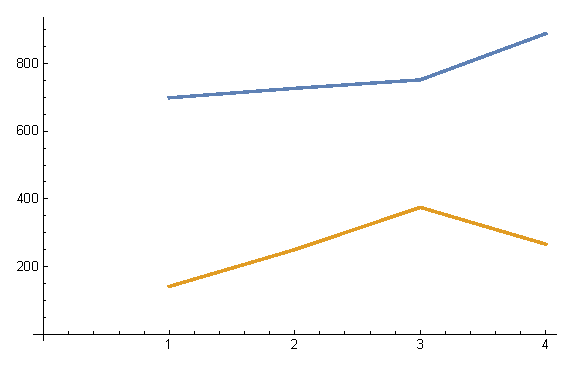
\includegraphics{plot.eps}
		\caption{The plots of the data measures.}
		\label{figure-4}
	\end{figure}

	From Figure \ref{figure-4} we can obviously tell the time cost of the reasoning increases by the round, as more reflections are inserted into the database. It should be noted that\DIFaddbegin \DIFadd{, }\DIFaddend for time reasons, the reduction algorithm is not implemented in this version of DefQed, and the coding quality can also be further improved.

	The experiment is done on a Hewlett-Packard ZBook mobile workstation 14u G5 \cite{HP-2018}. During the experiment, all the programs/applications not necessary are closed except for the terminal emulator (ConEmu) and the program to benchmark. The operating system is Microsoft Windows 11 Pro for Workstations Insider Preview (Build 25211). The processor is Intel Core i5 8250U and the memory size is 8.0 GB\DIFdelbegin \DIFdel{installed}\DIFdelend . We used Wolfram Language version 12.0 and DefQed version 0.03. As DefQed utilizes MySQL as its database, it is necessary to point out we are using MySQL version 8.0 (Community). The DefQed source code is built with option `Release Mode' for Microsoft Windows x64 processor with .NET 6.0 platform.

	We also need to point out that\DIFaddbegin \DIFadd{, }\DIFaddend though in each round DefQed seems to be slower than others, it does not mean that the algorithm has a worse efficiency and performance when comparing to others. The performance difference between platform and programming language utilized by the two, NET and mainly C contributes to the difference of the two applications, not mentioning that while Wolfram Engine can only prove equations, DefQed is a generic approach. The quality of the optimization of the codes are also not on be same basis.

	\section{Conclusions and future work}

	In the sections before we have presented an elegant data structure for representing mathematical concepts and a neat process which utilizes category theory concepts and knowledge to conduct \DIFdelbegin \DIFdel{proof}\DIFdelend \DIFaddbegin \DIFadd{proofs}\DIFaddend , which also have self-optimization features.

	Currently\DIFaddbegin \DIFadd{, }\DIFaddend we have developed a computer program called DefQed that implements the algorithm and it is open-sourced with BSD 3-Clause {``}New{''} or {``}Revised{''} License on GitHub. The source code of the latest version can be accessed at \cite{Wang2022}\DIFaddbegin \DIFadd{. }\DIFaddend It should be noted that the version is very early and some aspects of the algorithm we presented in the paper \DIFdelbegin \DIFdel{is }\DIFdelend \DIFaddbegin \DIFadd{are }\DIFaddend not implemented.

	Future works are the followings below:
	\begin{itemize}
		\item \textbf{Continuing the implementation of the corresponding software.} Currently\DIFaddbegin \DIFadd{, }\DIFaddend the software we developed is still under \DIFdelbegin \DIFdel{immature }\DIFdelend \DIFaddbegin \DIFadd{early }\DIFaddend development and a great many of the aspects we presented in the paper above, including the self-evolution logic, have not been constructed yet.
		\item  \textbf{Improving the algorithm.} The algorithm we presented in the paper is not mature. For instance, if the knowledge base has more than \(2^{32}\) morphisms, then some of the morphisms will never be utilized.
		\item \textbf{Optimizing the algorithm.} Currently, though the design of the procedures increase generality because of the low-knowledge feature, the performance of derivations may be lower than the current algorithms, which focus on a certain subject inside mathematics.
	\end{itemize}

	\section*{Acknowledgments}
	I express my sincerest gratitude to my tutor Prof. Shao Xinhui, the Yingcai Project of China, which enables senior high school students to conduct science research, my senior high academy Northeast Yucai School (NEYC) of China and the corresponding university Northern Eastern University (NEU) of China. I also thank my parents for encouraging me to conduct this research project. Additionally, I had \DIFdelbegin \DIFdel{few }\DIFdelend \DIFaddbegin \DIFadd{little }\DIFaddend knowledge about \LaTeX before writing this paper. The $lshort$ documentation and the \TeX Stack Exchange helped me a lot. Here I express my genuine thankfulness to the online resources and documentation of the used \LaTeX packages and software components. 

	 This research \DIFdelbegin \DIFdel{receive }\DIFdelend \DIFaddbegin \DIFadd{received }\DIFaddend general aid from the Yingcai Project of China.

	\section*{Conflict of interests}

	The authors declare no conflict of interest.

\begin{thebibliography}{999}

\bibitem[Wolfram(2019)]{Wolfram2019}
S. Wolfram,
 \emph{Wolfram language \& system documentation center},
 Wolfram Research Inc., Champaign, IL, US, 12.0 Eds, 2019.

\bibitem[Gao(1998)]{Gao1998}
X. S. Gao,
 {\it Geoexpert}, Beijing, 1998.
 Available from:
  \url{http://www.mmrc.iss.ac.cn/gex/}.

\bibitem[Moura and Ullrich(2021)]{Moura2021}
L.~D. Moura, S. Ullrich,
 The lean 4 theorem prover and programming language,
 \emph{Autom. Deduction -CADE}, 2021, 625--235. 
 \doilink{http://doi.org/10.1007/978-3-030-79876-5_37}

 
\bibitem[Moura and Bjørner(2008)]{Moura2008}
L.~D. Moura, N.~Bjørner,
 {\it Z3: An efficient smt solver,}
 in {Tools and Algorithms for the Construction and Analysis of
  Systems}, {\bf 4963} (2008), 337--340.
 \doilink{http://doi.org/10.1007/978-3-540-78800-3\_24}
\bibitem[Li(2019)]{Li2019}
W. W. Li,
 \emph{Daishuxue Fangfa}, 1 Ed, 
 High Education Press, Beijing, 2019.
 ISBN 978-7-04-050725-6.

\bibitem[Ebbinghaus(1913)]{Ebbinghaus1913}
H. Ebbinghaus,
 \emph{Memory: A contribution to experimental psychology},
 Teachers College, Columbia University, New York City, 1913.
 Available from:
  \url{https://archive.org/details/memorycontributi00ebbiuoft/page/n5/mode/2up}.

\bibitem[Entacher(1997)]{Entacher1997}
K.~Entacher,
 A collection of selected pseudorandom number generators with linear structures, 1997.
 Available from:
  \url{https://www.semanticscholar.org/paper/6ae5fe88d296e70f188b0d12207d468c8f36e262}.

\bibitem[Tanenbaum(2015)]{Tanenbaum2015}
A.~S. Tanenbaum,
 \emph{Operating systems: Design and implementation (volume~1)}, 
 Publishing House of Electronics Industry, Beijing, 3 Eds, 2015.
 ISBN 978-7-121-26193-0.

\bibitem[Wang(2022{\natexlab{a}})]{Wang2022}
Z. J. Wang,
 The defqed repository, 
2022.
 Available from: \url{https://github.com/ZijianFelixWang/DefQed}.

\bibitem[Wang(2022{\natexlab{b}})]{Wang2022-2}
Z. J. Wang,
 Benchmark of the defqed algorithm, 2022.
 Available from: \url{https://github.com/ZijianFelixWang/DefQed-Benchmark}.

\bibitem[Hewlett-Packard(2018)]{HP-2018}
H. Packard,
 {\it The hp zbook 14u g5 specifications}, 2018. 
 \url{https://support.hp.com/us-en/document/c05873311}. 


\end{thebibliography}

	
	

\end{document}
